\documentclass[]{article}
\usepackage{lmodern}
\usepackage{amssymb,amsmath}
\usepackage{ifxetex,ifluatex}
\usepackage{fixltx2e} % provides \textsubscript
\ifnum 0\ifxetex 1\fi\ifluatex 1\fi=0 % if pdftex
  \usepackage[T1]{fontenc}
  \usepackage[utf8]{inputenc}
\else % if luatex or xelatex
  \ifxetex
    \usepackage{mathspec}
  \else
    \usepackage{fontspec}
  \fi
  \defaultfontfeatures{Ligatures=TeX,Scale=MatchLowercase}
\fi
% use upquote if available, for straight quotes in verbatim environments
\IfFileExists{upquote.sty}{\usepackage{upquote}}{}
% use microtype if available
\IfFileExists{microtype.sty}{%
\usepackage{microtype}
\UseMicrotypeSet[protrusion]{basicmath} % disable protrusion for tt fonts
}{}
\usepackage[margin=2.54cm]{geometry}
\usepackage{hyperref}
\hypersetup{unicode=true,
            pdftitle={9: Data Visualization},
            pdfauthor={Environmental Data Analytics \textbar{} Kateri Salk},
            pdfborder={0 0 0},
            breaklinks=true}
\urlstyle{same}  % don't use monospace font for urls
\usepackage{color}
\usepackage{fancyvrb}
\newcommand{\VerbBar}{|}
\newcommand{\VERB}{\Verb[commandchars=\\\{\}]}
\DefineVerbatimEnvironment{Highlighting}{Verbatim}{commandchars=\\\{\}}
% Add ',fontsize=\small' for more characters per line
\usepackage{framed}
\definecolor{shadecolor}{RGB}{248,248,248}
\newenvironment{Shaded}{\begin{snugshade}}{\end{snugshade}}
\newcommand{\KeywordTok}[1]{\textcolor[rgb]{0.13,0.29,0.53}{\textbf{#1}}}
\newcommand{\DataTypeTok}[1]{\textcolor[rgb]{0.13,0.29,0.53}{#1}}
\newcommand{\DecValTok}[1]{\textcolor[rgb]{0.00,0.00,0.81}{#1}}
\newcommand{\BaseNTok}[1]{\textcolor[rgb]{0.00,0.00,0.81}{#1}}
\newcommand{\FloatTok}[1]{\textcolor[rgb]{0.00,0.00,0.81}{#1}}
\newcommand{\ConstantTok}[1]{\textcolor[rgb]{0.00,0.00,0.00}{#1}}
\newcommand{\CharTok}[1]{\textcolor[rgb]{0.31,0.60,0.02}{#1}}
\newcommand{\SpecialCharTok}[1]{\textcolor[rgb]{0.00,0.00,0.00}{#1}}
\newcommand{\StringTok}[1]{\textcolor[rgb]{0.31,0.60,0.02}{#1}}
\newcommand{\VerbatimStringTok}[1]{\textcolor[rgb]{0.31,0.60,0.02}{#1}}
\newcommand{\SpecialStringTok}[1]{\textcolor[rgb]{0.31,0.60,0.02}{#1}}
\newcommand{\ImportTok}[1]{#1}
\newcommand{\CommentTok}[1]{\textcolor[rgb]{0.56,0.35,0.01}{\textit{#1}}}
\newcommand{\DocumentationTok}[1]{\textcolor[rgb]{0.56,0.35,0.01}{\textbf{\textit{#1}}}}
\newcommand{\AnnotationTok}[1]{\textcolor[rgb]{0.56,0.35,0.01}{\textbf{\textit{#1}}}}
\newcommand{\CommentVarTok}[1]{\textcolor[rgb]{0.56,0.35,0.01}{\textbf{\textit{#1}}}}
\newcommand{\OtherTok}[1]{\textcolor[rgb]{0.56,0.35,0.01}{#1}}
\newcommand{\FunctionTok}[1]{\textcolor[rgb]{0.00,0.00,0.00}{#1}}
\newcommand{\VariableTok}[1]{\textcolor[rgb]{0.00,0.00,0.00}{#1}}
\newcommand{\ControlFlowTok}[1]{\textcolor[rgb]{0.13,0.29,0.53}{\textbf{#1}}}
\newcommand{\OperatorTok}[1]{\textcolor[rgb]{0.81,0.36,0.00}{\textbf{#1}}}
\newcommand{\BuiltInTok}[1]{#1}
\newcommand{\ExtensionTok}[1]{#1}
\newcommand{\PreprocessorTok}[1]{\textcolor[rgb]{0.56,0.35,0.01}{\textit{#1}}}
\newcommand{\AttributeTok}[1]{\textcolor[rgb]{0.77,0.63,0.00}{#1}}
\newcommand{\RegionMarkerTok}[1]{#1}
\newcommand{\InformationTok}[1]{\textcolor[rgb]{0.56,0.35,0.01}{\textbf{\textit{#1}}}}
\newcommand{\WarningTok}[1]{\textcolor[rgb]{0.56,0.35,0.01}{\textbf{\textit{#1}}}}
\newcommand{\AlertTok}[1]{\textcolor[rgb]{0.94,0.16,0.16}{#1}}
\newcommand{\ErrorTok}[1]{\textcolor[rgb]{0.64,0.00,0.00}{\textbf{#1}}}
\newcommand{\NormalTok}[1]{#1}
\usepackage{graphicx,grffile}
\makeatletter
\def\maxwidth{\ifdim\Gin@nat@width>\linewidth\linewidth\else\Gin@nat@width\fi}
\def\maxheight{\ifdim\Gin@nat@height>\textheight\textheight\else\Gin@nat@height\fi}
\makeatother
% Scale images if necessary, so that they will not overflow the page
% margins by default, and it is still possible to overwrite the defaults
% using explicit options in \includegraphics[width, height, ...]{}
\setkeys{Gin}{width=\maxwidth,height=\maxheight,keepaspectratio}
\IfFileExists{parskip.sty}{%
\usepackage{parskip}
}{% else
\setlength{\parindent}{0pt}
\setlength{\parskip}{6pt plus 2pt minus 1pt}
}
\setlength{\emergencystretch}{3em}  % prevent overfull lines
\providecommand{\tightlist}{%
  \setlength{\itemsep}{0pt}\setlength{\parskip}{0pt}}
\setcounter{secnumdepth}{0}
% Redefines (sub)paragraphs to behave more like sections
\ifx\paragraph\undefined\else
\let\oldparagraph\paragraph
\renewcommand{\paragraph}[1]{\oldparagraph{#1}\mbox{}}
\fi
\ifx\subparagraph\undefined\else
\let\oldsubparagraph\subparagraph
\renewcommand{\subparagraph}[1]{\oldsubparagraph{#1}\mbox{}}
\fi

%%% Use protect on footnotes to avoid problems with footnotes in titles
\let\rmarkdownfootnote\footnote%
\def\footnote{\protect\rmarkdownfootnote}

%%% Change title format to be more compact
\usepackage{titling}

% Create subtitle command for use in maketitle
\newcommand{\subtitle}[1]{
  \posttitle{
    \begin{center}\large#1\end{center}
    }
}

\setlength{\droptitle}{-2em}

  \title{9: Data Visualization}
    \pretitle{\vspace{\droptitle}\centering\huge}
  \posttitle{\par}
    \author{Environmental Data Analytics \textbar{} Kateri Salk}
    \preauthor{\centering\large\emph}
  \postauthor{\par}
      \predate{\centering\large\emph}
  \postdate{\par}
    \date{Spring 2019}


\begin{document}
\maketitle

\subsection{LESSON OBJECTIVES}\label{lesson-objectives}

\begin{enumerate}
\def\labelenumi{\arabic{enumi}.}
\tightlist
\item
  Perform simple data visualizations in the R package \texttt{ggplot}
\item
  Develop skills to adjust aesthetics and layers in graphs
\item
  Apply a decision tree framework for appropriate graphing methods
\end{enumerate}

\subsection{SET UP YOUR DATA ANALYSIS
SESSION}\label{set-up-your-data-analysis-session}

\begin{Shaded}
\begin{Highlighting}[]
\KeywordTok{getwd}\NormalTok{()}
\end{Highlighting}
\end{Shaded}

\begin{verbatim}
## [1] "C:/Users/Felipe/OneDrive - Duke University/1. DUKE/1. Ramos 2 Semestre/EOS-872 Env. Data Analytics/Environmental_Data_Analytics"
\end{verbatim}

\begin{Shaded}
\begin{Highlighting}[]
\KeywordTok{library}\NormalTok{(tidyverse) }\CommentTok{#ggplot is included here}

\NormalTok{PeterPaul.chem.nutrients <-}\StringTok{ }\KeywordTok{read.csv}\NormalTok{(}\StringTok{"./Data/Processed/NTL-LTER_Lake_Chemistry_Nutrients_PeterPaul_Processed.csv"}\NormalTok{)}
\NormalTok{PeterPaul.nutrients.gathered <-}\StringTok{ }\KeywordTok{read.csv}\NormalTok{(}\StringTok{"./Data/Processed/NTL-LTER_Lake_Nutrients_PeterPaulGathered_Processed.csv"}\NormalTok{)}
\NormalTok{PeterPaul.chem.nutrients.summaries <-}\StringTok{ }\KeywordTok{read.csv}\NormalTok{(}\StringTok{"./Data/Processed/NTL-LTER_Lake_Summaries_PeterPaul_Processed.csv"}\NormalTok{)}
\NormalTok{EPAair <-}\StringTok{ }\KeywordTok{read.csv}\NormalTok{(}\StringTok{"./Data/Processed/EPAair_O3_PM25_NC1718_Processed.csv"}\NormalTok{)}

\NormalTok{EPAair}\OperatorTok{$}\NormalTok{Date <-}\StringTok{ }\KeywordTok{as.Date}\NormalTok{(EPAair}\OperatorTok{$}\NormalTok{Date, }\DataTypeTok{format =} \StringTok{"%Y-%m-%d"}\NormalTok{) }\CommentTok{#we always need to do the date thing again}
\NormalTok{PeterPaul.chem.nutrients}\OperatorTok{$}\NormalTok{sampledate <-}\StringTok{ }\KeywordTok{as.Date}\NormalTok{(PeterPaul.chem.nutrients}\OperatorTok{$}\NormalTok{sampledate, }\DataTypeTok{format =} \StringTok{"%Y-%m-%d"}\NormalTok{) }\CommentTok{#we always need to do the date thing again Lubridate also can format dates.}
\end{Highlighting}
\end{Shaded}

\subsection{GGPLOT}\label{ggplot}

ggplot, called from the package \texttt{ggplot2}, is a graphing and
image generation tool in R. This package is part of tidyverse. While
base R has graphing capabilities, ggplot has the capacity for a wider
range and more sophisticated options for graphing. ggplot has only a few
rules:

\begin{itemize}
\tightlist
\item
  The first line of ggplot code always starts with \texttt{ggplot()}
\item
  A data frame must be specified within the \texttt{ggplot()} function.
  Additional datasets can be specified in subsequent layers.
\item
  Aesthetics must be specified, most commonly x and y variables but
  including others. Aesthetics can be specified in the \texttt{ggplot()}
  function or in subsequent layers.
\item
  Additional layers must be specified to fill the plot.
\end{itemize}

\subsubsection{Geoms \#sometimes you can use other dataframes in the
geom}\label{geoms-sometimes-you-can-use-other-dataframes-in-the-geom}

Here are some commonly used layers for plotting in ggplot:

\begin{itemize}
\tightlist
\item
  geom\_bar
\item
  geom\_histogram
\item
  geom\_freqpoly
\item
  geom\_boxplot
\item
  geom\_violin
\item
  geom\_dotplot
\item
  geom\_point
\item
  geom\_errorbar
\item
  geom\_smooth
\item
  geom\_line
\item
  geom\_area
\item
  geom\_abline (plus geom\_hline and geom\_vline)
\item
  geom\_text
\end{itemize}

\subsubsection{Aesthetics}\label{aesthetics}

Here are some commonly used aesthetic types that can be manipulated in
ggplot:

\begin{itemize}
\tightlist
\item
  color
\item
  fill
\item
  shape
\item
  size
\item
  transparency
\end{itemize}

\subsubsection{Plotting continuous variables over time:
Scatterplot}\label{plotting-continuous-variables-over-time-scatterplot}

\begin{Shaded}
\begin{Highlighting}[]
\CommentTok{# Scatterplot}
\KeywordTok{ggplot}\NormalTok{(EPAair, }\KeywordTok{aes}\NormalTok{(}\DataTypeTok{x =}\NormalTok{ Date, }\DataTypeTok{y =}\NormalTok{ Ozone)) }\OperatorTok{+}\StringTok{ }
\StringTok{  }\KeywordTok{geom_point}\NormalTok{()}
\end{Highlighting}
\end{Shaded}

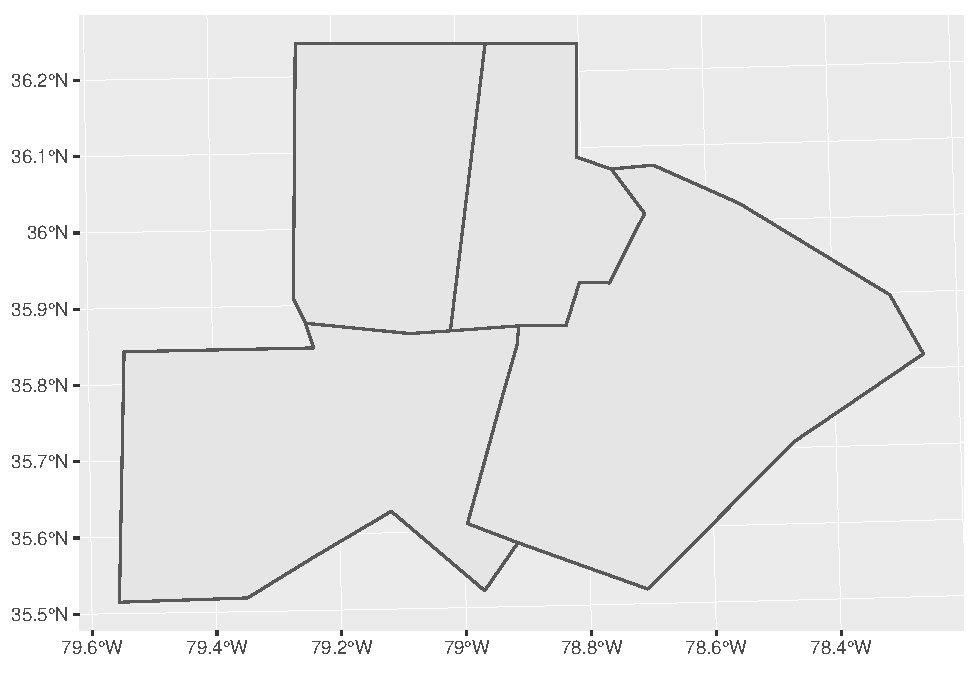
\includegraphics{09_DataVisualization_files/figure-latex/unnamed-chunk-2-1.pdf}

\begin{Shaded}
\begin{Highlighting}[]
\NormalTok{O3plot <-}\StringTok{ }\KeywordTok{ggplot}\NormalTok{(EPAair) }\OperatorTok{+}
\StringTok{  }\KeywordTok{geom_point}\NormalTok{(}\KeywordTok{aes}\NormalTok{(}\DataTypeTok{x =}\NormalTok{ Date, }\DataTypeTok{y =}\NormalTok{ Ozone))}
\KeywordTok{print}\NormalTok{(O3plot) }\CommentTok{# you get the same result. Print() prints it in a pdf.}
\end{Highlighting}
\end{Shaded}

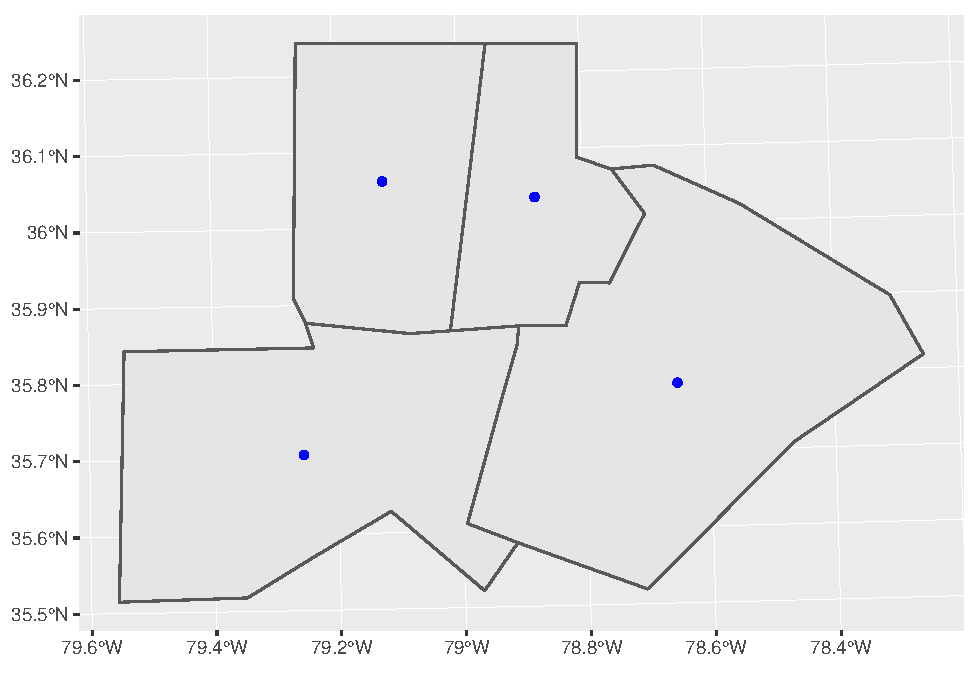
\includegraphics{09_DataVisualization_files/figure-latex/unnamed-chunk-2-2.pdf}

\begin{Shaded}
\begin{Highlighting}[]
\CommentTok{# Fix this code}
\NormalTok{O3plot2 <-}\StringTok{ }\KeywordTok{ggplot}\NormalTok{(EPAair) }\OperatorTok{+}
\StringTok{  }\KeywordTok{geom_point}\NormalTok{(}\KeywordTok{aes}\NormalTok{(}\DataTypeTok{x =}\NormalTok{ Date, }\DataTypeTok{y =}\NormalTok{ Ozone), }\DataTypeTok{color =} \StringTok{"blue"}\NormalTok{) }\CommentTok{# fixed}
\KeywordTok{print}\NormalTok{(O3plot2)}
\end{Highlighting}
\end{Shaded}

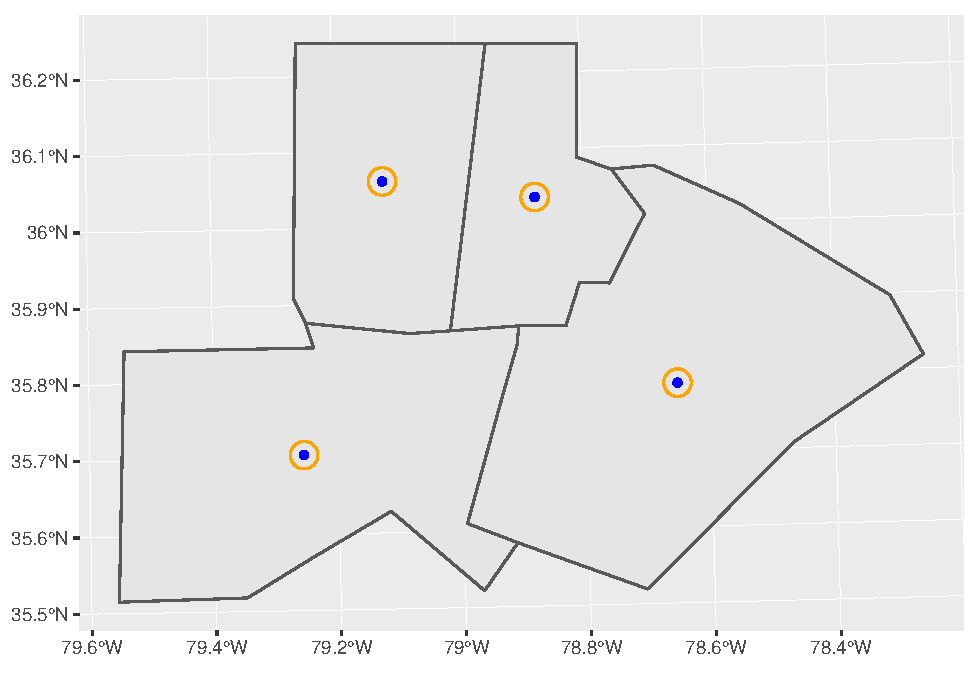
\includegraphics{09_DataVisualization_files/figure-latex/unnamed-chunk-2-3.pdf}

\begin{Shaded}
\begin{Highlighting}[]
\CommentTok{# Add additional variables}
\NormalTok{PMplot <-}\StringTok{ }
\StringTok{  }\KeywordTok{ggplot}\NormalTok{(EPAair, }\KeywordTok{aes}\NormalTok{(}\DataTypeTok{x =} \KeywordTok{as.factor}\NormalTok{(Month), }\DataTypeTok{y =}\NormalTok{ PM25, }\DataTypeTok{shape =} \KeywordTok{as.factor}\NormalTok{(Year), }\DataTypeTok{color =}\NormalTok{ Site.Name)) }\OperatorTok{+}
\StringTok{  }\KeywordTok{geom_point}\NormalTok{() }\CommentTok{# here makes sense color inside aes # month goes to 12.5. not pretty. as factor solves it }
\KeywordTok{print}\NormalTok{(PMplot)}
\end{Highlighting}
\end{Shaded}

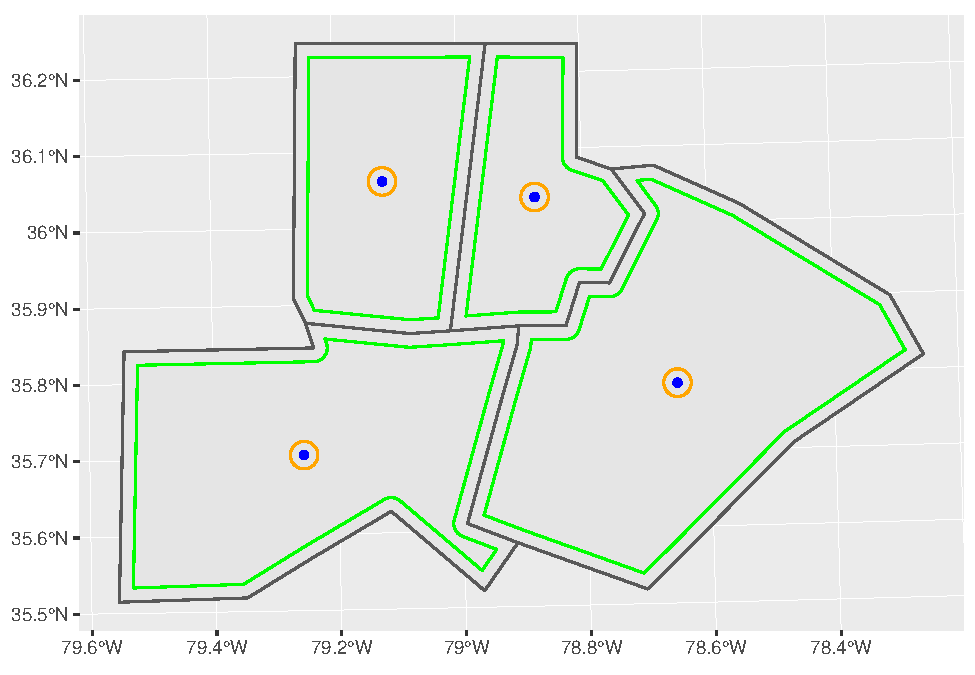
\includegraphics{09_DataVisualization_files/figure-latex/unnamed-chunk-2-4.pdf}

\begin{Shaded}
\begin{Highlighting}[]
\CommentTok{# Separate plot with facets}
\NormalTok{PMplot.faceted <-}
\StringTok{  }\KeywordTok{ggplot}\NormalTok{(EPAair, }\KeywordTok{aes}\NormalTok{(}\DataTypeTok{x =}\NormalTok{ Month, }\DataTypeTok{y =}\NormalTok{ PM25, }\DataTypeTok{shape =} \KeywordTok{as.factor}\NormalTok{(Year))) }\OperatorTok{+}
\StringTok{  }\KeywordTok{geom_point}\NormalTok{() }\OperatorTok{+}
\StringTok{  }\KeywordTok{facet_wrap}\NormalTok{(}\KeywordTok{vars}\NormalTok{(Site.Name)) }\CommentTok{#new layer. three rows. three graphs. if not default is columns.}
\KeywordTok{print}\NormalTok{(PMplot.faceted)}
\end{Highlighting}
\end{Shaded}

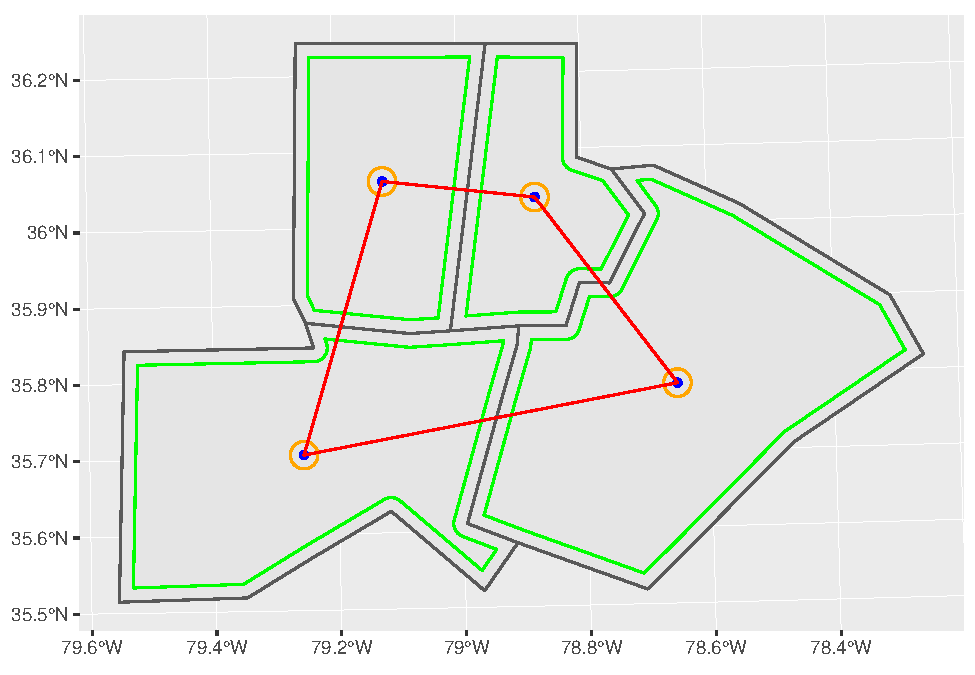
\includegraphics{09_DataVisualization_files/figure-latex/unnamed-chunk-2-5.pdf}

\begin{Shaded}
\begin{Highlighting}[]
\NormalTok{PMplot.faceted2 <-}
\StringTok{  }\KeywordTok{ggplot}\NormalTok{(EPAair, }\KeywordTok{aes}\NormalTok{(}\DataTypeTok{x =}\NormalTok{ Month, }\DataTypeTok{y =}\NormalTok{ PM25)) }\OperatorTok{+}
\StringTok{  }\KeywordTok{geom_point}\NormalTok{() }\OperatorTok{+}
\StringTok{  }\KeywordTok{facet_grid}\NormalTok{(Site.Name }\OperatorTok{~}\StringTok{ }\NormalTok{Year) }\CommentTok{# tilda is by}
\KeywordTok{print}\NormalTok{(PMplot.faceted2)}
\end{Highlighting}
\end{Shaded}

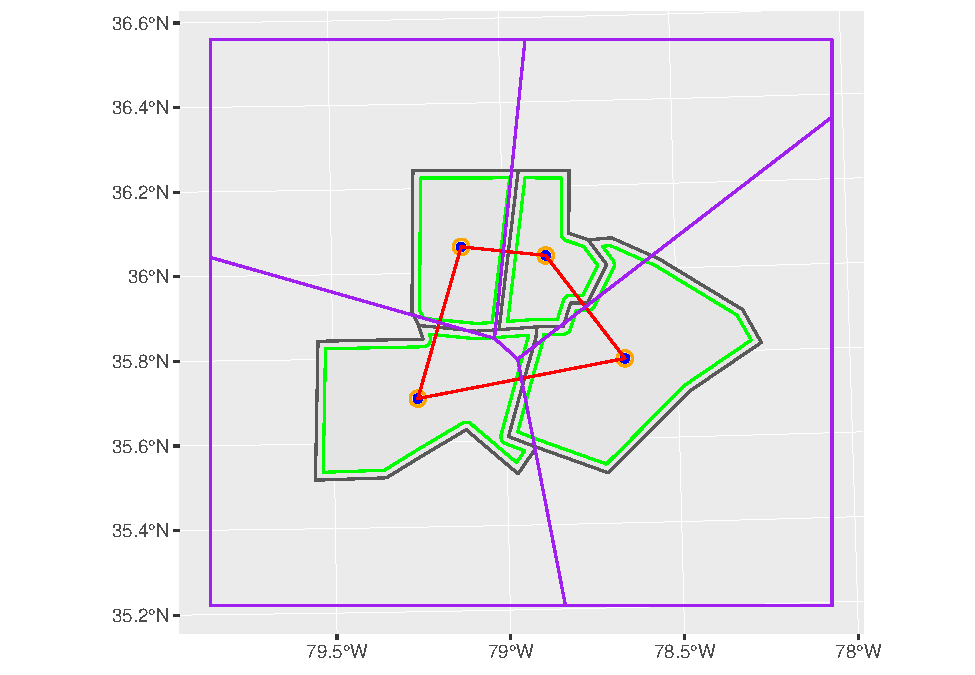
\includegraphics{09_DataVisualization_files/figure-latex/unnamed-chunk-2-6.pdf}

\begin{Shaded}
\begin{Highlighting}[]
\CommentTok{# Filter dataset within plot building}
\NormalTok{O3plot.Blackstone <-}\StringTok{ }
\StringTok{  }\KeywordTok{ggplot}\NormalTok{(}\KeywordTok{subset}\NormalTok{(EPAair, Site.Name }\OperatorTok{==}\StringTok{ "Blackstone"}\NormalTok{), }\KeywordTok{aes}\NormalTok{(}\DataTypeTok{x =}\NormalTok{ Date, }\DataTypeTok{y =}\NormalTok{ Ozone)) }\OperatorTok{+}\StringTok{ }
\StringTok{  }\KeywordTok{geom_point}\NormalTok{() }\OperatorTok{+}
\StringTok{  }\KeywordTok{geom_line}\NormalTok{() }\CommentTok{# puts a line between the dots}
\KeywordTok{print}\NormalTok{(O3plot.Blackstone) }\CommentTok{#subset of only Blackstone}
\end{Highlighting}
\end{Shaded}

\includegraphics{09_DataVisualization_files/figure-latex/unnamed-chunk-2-7.pdf}

\begin{Shaded}
\begin{Highlighting}[]
\CommentTok{# Exercise: build your own scatterplots of PeterPaul.chem.nutrients}

\CommentTok{# 1. }
\CommentTok{# Plot surface temperatures by day of  year. }
\CommentTok{# Color your points by year, and facet by lake in two rows.}

\NormalTok{PeterPaul.chem.nutrients.faceted <-}
\StringTok{  }\KeywordTok{ggplot}\NormalTok{(PeterPaul.chem.nutrients, }\KeywordTok{aes}\NormalTok{(}\DataTypeTok{x =}\NormalTok{ daynum, }\DataTypeTok{y =}\NormalTok{ temperature_C, }\DataTypeTok{color =}\NormalTok{ year4)) }\OperatorTok{+}
\StringTok{  }\KeywordTok{geom_point}\NormalTok{() }\OperatorTok{+}
\StringTok{  }\KeywordTok{facet_wrap}\NormalTok{(}\KeywordTok{vars}\NormalTok{(lakename), }\DataTypeTok{nrow =} \DecValTok{2}\NormalTok{) }
\KeywordTok{print}\NormalTok{(PeterPaul.chem.nutrients.faceted)}
\end{Highlighting}
\end{Shaded}

\includegraphics{09_DataVisualization_files/figure-latex/unnamed-chunk-2-8.pdf}

\begin{Shaded}
\begin{Highlighting}[]
\CommentTok{#2. }
\CommentTok{# Plot temperature by date. Color your points by depth.}
\CommentTok{# Change the size of your point to 0.5}

\NormalTok{PeterPaul.chem.nutrients.faceted2 <-}
\StringTok{  }\KeywordTok{ggplot}\NormalTok{(PeterPaul.chem.nutrients, }\KeywordTok{aes}\NormalTok{(}\DataTypeTok{x =}\NormalTok{ sampledate, }\DataTypeTok{y =}\NormalTok{ temperature_C, }\DataTypeTok{color =}\NormalTok{ depth)) }\OperatorTok{+}
\StringTok{  }\KeywordTok{geom_point}\NormalTok{(}\DataTypeTok{size =} \FloatTok{0.5}\NormalTok{)}
  \KeywordTok{print}\NormalTok{(PeterPaul.chem.nutrients.faceted2)}
\end{Highlighting}
\end{Shaded}

\includegraphics{09_DataVisualization_files/figure-latex/unnamed-chunk-2-9.pdf}
\#\#\# Plotting the relationship between two continuous variables:
Scatterplot

\begin{Shaded}
\begin{Highlighting}[]
\CommentTok{# Scatterplot}
\NormalTok{lightvsDO <-}\StringTok{ }
\StringTok{  }\KeywordTok{ggplot}\NormalTok{(PeterPaul.chem.nutrients, }\KeywordTok{aes}\NormalTok{(}\DataTypeTok{x =}\NormalTok{ irradianceWater, }\DataTypeTok{y =}\NormalTok{ dissolvedOxygen)) }\OperatorTok{+}
\StringTok{  }\KeywordTok{geom_point}\NormalTok{()}
\KeywordTok{print}\NormalTok{(lightvsDO)}
\end{Highlighting}
\end{Shaded}

\includegraphics{09_DataVisualization_files/figure-latex/unnamed-chunk-3-1.pdf}

\begin{Shaded}
\begin{Highlighting}[]
\CommentTok{# Adjust axes}
\NormalTok{lightvsDOfixed <-}\StringTok{ }
\StringTok{  }\KeywordTok{ggplot}\NormalTok{(PeterPaul.chem.nutrients, }\KeywordTok{aes}\NormalTok{(}\DataTypeTok{x =}\NormalTok{ irradianceWater, }\DataTypeTok{y =}\NormalTok{ dissolvedOxygen)) }\OperatorTok{+}
\StringTok{  }\KeywordTok{geom_point}\NormalTok{() }\OperatorTok{+}
\StringTok{  }\KeywordTok{xlim}\NormalTok{(}\DecValTok{0}\NormalTok{, }\DecValTok{250}\NormalTok{) }\OperatorTok{+}\StringTok{ }\CommentTok{# we set our axis to known data normal limits.}
\StringTok{  }\KeywordTok{ylim}\NormalTok{(}\DecValTok{0}\NormalTok{, }\DecValTok{20}\NormalTok{)}
\KeywordTok{print}\NormalTok{(lightvsDOfixed)}
\end{Highlighting}
\end{Shaded}

\includegraphics{09_DataVisualization_files/figure-latex/unnamed-chunk-3-2.pdf}

\begin{Shaded}
\begin{Highlighting}[]
\CommentTok{# Depth in the fields of limnology and oceanography is on a reverse scale}
\NormalTok{tempvsdepth <-}\StringTok{ }
\StringTok{  }\CommentTok{#ggplot(PeterPaul.chem.nutrients, aes(x = temperature_C, y = depth)) +}
\StringTok{  }\KeywordTok{ggplot}\NormalTok{(PeterPaul.chem.nutrients, }\KeywordTok{aes}\NormalTok{(}\DataTypeTok{x =}\NormalTok{ temperature_C, }\DataTypeTok{y =}\NormalTok{ depth, }\DataTypeTok{color =}\NormalTok{ daynum)) }\OperatorTok{+}
\StringTok{  }\KeywordTok{geom_point}\NormalTok{() }\OperatorTok{+}
\StringTok{  }\KeywordTok{scale_y_reverse}\NormalTok{()    }\CommentTok{#Reverse Axis}
\KeywordTok{print}\NormalTok{(tempvsdepth)}
\end{Highlighting}
\end{Shaded}

\includegraphics{09_DataVisualization_files/figure-latex/unnamed-chunk-3-3.pdf}

\begin{Shaded}
\begin{Highlighting}[]
\CommentTok{#CLASS 2 ###########################################################################}
\NormalTok{NvsP <-}
\StringTok{  }\KeywordTok{ggplot}\NormalTok{(PeterPaul.chem.nutrients, }\KeywordTok{aes}\NormalTok{(}\DataTypeTok{x =}\NormalTok{ tp_ug, }\DataTypeTok{y =}\NormalTok{ tn_ug, }\DataTypeTok{color =}\NormalTok{ depth)) }\OperatorTok{+}
\StringTok{  }\KeywordTok{geom_point}\NormalTok{() }\OperatorTok{+}
\StringTok{  }\KeywordTok{geom_smooth}\NormalTok{(}\DataTypeTok{method =}\NormalTok{ lm) }\OperatorTok{+}\StringTok{ }\CommentTok{#without the inside uses smooth function}
\StringTok{  }\KeywordTok{geom_abline}\NormalTok{(}\KeywordTok{aes}\NormalTok{(}\DataTypeTok{slope =} \DecValTok{16}\NormalTok{, }\DataTypeTok{intercept =} \DecValTok{0}\NormalTok{), }\DataTypeTok{lty =} \DecValTok{2}\NormalTok{) }\CommentTok{# lty = linetype. The points are above the line. We have more nitrogen than phosphorus. Typical in the US.}
\KeywordTok{print}\NormalTok{(NvsP)   }\CommentTok{# there are grey points. points with no value for the color.}
\end{Highlighting}
\end{Shaded}

\includegraphics{09_DataVisualization_files/figure-latex/unnamed-chunk-3-4.pdf}

\begin{Shaded}
\begin{Highlighting}[]
\CommentTok{# Exercise: Plot relationships between air quality measurements}

\CommentTok{# 1. }
\CommentTok{# Plot AQI values for ozone by PM2.5, colored by site. }

\NormalTok{O3vsPM25 <-}
\StringTok{  }\KeywordTok{ggplot}\NormalTok{(EPAair, }\KeywordTok{aes}\NormalTok{(}\DataTypeTok{x =}\NormalTok{ PM25, }\DataTypeTok{y =}\NormalTok{ Ozone, }\DataTypeTok{color =}\NormalTok{ Site.Name)) }\OperatorTok{+}
\StringTok{  }\KeywordTok{geom_point}\NormalTok{() }\CommentTok{#+}
  \KeywordTok{geom_smooth}\NormalTok{(}\DataTypeTok{method =}\NormalTok{ lm) }\CommentTok{#+ }
\end{Highlighting}
\end{Shaded}

\begin{verbatim}
## geom_smooth: na.rm = FALSE, se = TRUE
## stat_smooth: na.rm = FALSE, se = TRUE, method = function (formula, data, subset, weights, na.action, method = "qr", model = TRUE, x = FALSE, y = FALSE, qr = TRUE, singular.ok = TRUE, contrasts = NULL, offset, ...) 
## {
##     ret.x <- x
##     ret.y <- y
##     cl <- match.call()
##     mf <- match.call(expand.dots = FALSE)
##     m <- match(c("formula", "data", "subset", "weights", "na.action", "offset"), names(mf), 0)
##     mf <- mf[c(1, m)]
##     mf$drop.unused.levels <- TRUE
##     mf[[1]] <- quote(stats::model.frame)
##     mf <- eval(mf, parent.frame())
##     if (method == "model.frame") 
##         return(mf)
##     else if (method != "qr") 
##         warning(gettextf("method = '%s' is not supported. Using 'qr'", method), domain = NA)
##     mt <- attr(mf, "terms")
##     y <- model.response(mf, "numeric")
##     w <- as.vector(model.weights(mf))
##     if (!is.null(w) && !is.numeric(w)) 
##         stop("'weights' must be a numeric vector")
##     offset <- as.vector(model.offset(mf))
##     if (!is.null(offset)) {
##         if (length(offset) != NROW(y)) 
##             stop(gettextf("number of offsets is %d, should equal %d (number of observations)", length(offset), NROW(y)), domain = NA)
##     }
##     if (is.empty.model(mt)) {
##         x <- NULL
##         z <- list(coefficients = if (is.matrix(y)) matrix(NA, 0, ncol(y)) else numeric(), residuals = y, fitted.values = 0 * y, weights = w, rank = 0, df.residual = if (!is.null(w)) sum(w != 0) else if (is.matrix(y)) nrow(y) else length(y))
##         if (!is.null(offset)) {
##             z$fitted.values <- offset
##             z$residuals <- y - offset
##         }
##     }
##     else {
##         x <- model.matrix(mt, mf, contrasts)
##         z <- if (is.null(w)) 
##             lm.fit(x, y, offset = offset, singular.ok = singular.ok, ...)
##         else lm.wfit(x, y, w, offset = offset, singular.ok = singular.ok, ...)
##     }
##     class(z) <- c(if (is.matrix(y)) "mlm", "lm")
##     z$na.action <- attr(mf, "na.action")
##     z$offset <- offset
##     z$contrasts <- attr(x, "contrasts")
##     z$xlevels <- .getXlevels(mt, mf)
##     z$call <- cl
##     z$terms <- mt
##     if (model) 
##         z$model <- mf
##     if (ret.x) 
##         z$x <- x
##     if (ret.y) 
##         z$y <- y
##     if (!qr) 
##         z$qr <- NULL
##     z
## }, formula = y ~ x
## position_identity
\end{verbatim}

\begin{Shaded}
\begin{Highlighting}[]
  \KeywordTok{geom_abline}\NormalTok{(}\KeywordTok{aes}\NormalTok{(}\DataTypeTok{slope =} \DecValTok{16}\NormalTok{, }\DataTypeTok{intercept =} \DecValTok{0}\NormalTok{), }\DataTypeTok{lty =} \DecValTok{2}\NormalTok{) }
\end{Highlighting}
\end{Shaded}

\begin{verbatim}
## mapping: slope = 16, intercept = 0 
## geom_abline: na.rm = FALSE
## stat_identity: na.rm = FALSE
## position_identity
\end{verbatim}

\begin{Shaded}
\begin{Highlighting}[]
\KeywordTok{print}\NormalTok{(O3vsPM25)}
\end{Highlighting}
\end{Shaded}

\includegraphics{09_DataVisualization_files/figure-latex/unnamed-chunk-3-5.pdf}

\begin{Shaded}
\begin{Highlighting}[]
\CommentTok{# Add a line of best fit for the linear regression of these variables.}
\NormalTok{O3vsPM25 <-}
\StringTok{  }\KeywordTok{ggplot}\NormalTok{(EPAair, }\KeywordTok{aes}\NormalTok{(}\DataTypeTok{x =}\NormalTok{ PM25, }\DataTypeTok{y =}\NormalTok{ Ozone, }\DataTypeTok{color =}\NormalTok{ Site.Name)) }\OperatorTok{+}
\StringTok{  }\KeywordTok{geom_point}\NormalTok{() }\OperatorTok{+}\StringTok{ }\CommentTok{# if you put here as(color=Site.Name) it gives one line for everything.}
\StringTok{  }\KeywordTok{geom_smooth}\NormalTok{(}\DataTypeTok{method =}\NormalTok{ lm) }\CommentTok{#+ }
  \KeywordTok{geom_abline}\NormalTok{(}\KeywordTok{aes}\NormalTok{(}\DataTypeTok{slope =} \DecValTok{16}\NormalTok{, }\DataTypeTok{intercept =} \DecValTok{0}\NormalTok{), }\DataTypeTok{lty =} \DecValTok{2}\NormalTok{) }
\end{Highlighting}
\end{Shaded}

\begin{verbatim}
## mapping: slope = 16, intercept = 0 
## geom_abline: na.rm = FALSE
## stat_identity: na.rm = FALSE
## position_identity
\end{verbatim}

\begin{Shaded}
\begin{Highlighting}[]
\KeywordTok{print}\NormalTok{(O3vsPM25)}
\end{Highlighting}
\end{Shaded}

\includegraphics{09_DataVisualization_files/figure-latex/unnamed-chunk-3-6.pdf}

\begin{Shaded}
\begin{Highlighting}[]
\KeywordTok{class}\NormalTok{(EPAair}\OperatorTok{$}\NormalTok{Site.Name)}
\end{Highlighting}
\end{Shaded}

\begin{verbatim}
## [1] "factor"
\end{verbatim}

\subsubsection{Plotting continuous vs.~categorical
variables}\label{plotting-continuous-vs.categorical-variables}

\begin{Shaded}
\begin{Highlighting}[]
 \CommentTok{# Barplot + error bars}
\NormalTok{PeterPaul.nutrient.summaries <-}\StringTok{ }\NormalTok{PeterPaul.nutrients.gathered }\OperatorTok
\StringTok{  }\KeywordTok{group_by}\NormalTok{(lakename, nutrient) }\OperatorTok\StringTok{   }\CommentTok{# we are grouping by two things}
\StringTok{  }\KeywordTok{summarise}\NormalTok{(}\DataTypeTok{sd =} \KeywordTok{sd}\NormalTok{(concentration), }
            \DataTypeTok{mean =} \KeywordTok{mean}\NormalTok{(concentration))}

\NormalTok{Nutrientplot <-}\StringTok{ }
\StringTok{  }\KeywordTok{ggplot}\NormalTok{(PeterPaul.nutrients.gathered) }\OperatorTok{+}
\StringTok{  }\KeywordTok{geom_bar}\NormalTok{(}\KeywordTok{aes}\NormalTok{(}\DataTypeTok{x =}\NormalTok{ lakename, }\DataTypeTok{y =}\NormalTok{ concentration, }\DataTypeTok{fill =}\NormalTok{ nutrient), }\CommentTok{# why did we use fill? Instead of color. Color only paints the border of the bars.}
           \DataTypeTok{position =} \StringTok{"dodge"}\NormalTok{, }\DataTypeTok{stat =} \StringTok{"summary"}\NormalTok{, }\DataTypeTok{fun.y =} \StringTok{"mean"}\NormalTok{)  }\CommentTok{# what's happening here? Dodge = stuck on top of each other. stat --> Summary --> mean}
\KeywordTok{print}\NormalTok{(Nutrientplot)}
\end{Highlighting}
\end{Shaded}

\includegraphics{09_DataVisualization_files/figure-latex/unnamed-chunk-4-1.pdf}

\begin{Shaded}
\begin{Highlighting}[]
\NormalTok{Nutrientplot2 <-}\StringTok{ }
\StringTok{  }\KeywordTok{ggplot}\NormalTok{(PeterPaul.nutrient.summaries, }\KeywordTok{aes}\NormalTok{(}\DataTypeTok{x =}\NormalTok{ lakename, }\DataTypeTok{y =}\NormalTok{ mean, }\DataTypeTok{fill =}\NormalTok{ nutrient)) }\OperatorTok{+}\StringTok{ }\CommentTok{#}
\StringTok{  }\KeywordTok{geom_bar}\NormalTok{(}\DataTypeTok{stat =} \StringTok{"identity"}\NormalTok{, }\DataTypeTok{position =} \StringTok{"dodge"}\NormalTok{) }\OperatorTok{+}\StringTok{ }\CommentTok{# what does the stat command do? The indentity of the cell. We already calculated the mean. You get to the same bar plot.}
\StringTok{  }\KeywordTok{geom_errorbar}\NormalTok{(}\KeywordTok{aes}\NormalTok{(}\DataTypeTok{ymin =}\NormalTok{ mean}\OperatorTok{-}\NormalTok{sd, }\DataTypeTok{ymax =}\NormalTok{ mean}\OperatorTok{+}\NormalTok{sd), }\CommentTok{# how do we specify error bars?}
                 \DataTypeTok{position =} \StringTok{"dodge"}\NormalTok{) }\CommentTok{#you need dodge}
\KeywordTok{print}\NormalTok{(Nutrientplot2) }\CommentTok{# not useful. Error goes below to zero. Not real value.}
\end{Highlighting}
\end{Shaded}

\includegraphics{09_DataVisualization_files/figure-latex/unnamed-chunk-4-2.pdf}

\begin{Shaded}
\begin{Highlighting}[]
\CommentTok{# Are there more effective ways to produce summary stats for categories? Alternatives-->}

\CommentTok{# Box and whiskers plot}
\NormalTok{Nutrientplot3 <-}
\StringTok{  }\KeywordTok{ggplot}\NormalTok{(PeterPaul.nutrients.gathered, }\KeywordTok{aes}\NormalTok{(}\DataTypeTok{x =}\NormalTok{ lakename, }\DataTypeTok{y =}\NormalTok{ concentration)) }\OperatorTok{+}
\StringTok{  }\KeywordTok{geom_boxplot}\NormalTok{(}\KeywordTok{aes}\NormalTok{(}\DataTypeTok{color =}\NormalTok{ nutrient)) }\CommentTok{# Why didn't we use "fill"? Dont wanna fill only the box plot}
\KeywordTok{print}\NormalTok{(Nutrientplot3)}
\end{Highlighting}
\end{Shaded}

\includegraphics{09_DataVisualization_files/figure-latex/unnamed-chunk-4-3.pdf}

\begin{Shaded}
\begin{Highlighting}[]
\CommentTok{# Dot plot}
\NormalTok{Nutrientplot4 <-}
\StringTok{  }\KeywordTok{ggplot}\NormalTok{(PeterPaul.nutrients.gathered, }\KeywordTok{aes}\NormalTok{(}\DataTypeTok{x =}\NormalTok{ lakename, }\DataTypeTok{y =}\NormalTok{ concentration)) }\OperatorTok{+}
\StringTok{  }\KeywordTok{geom_dotplot}\NormalTok{(}\KeywordTok{aes}\NormalTok{(}\DataTypeTok{color =}\NormalTok{ nutrient), }\DataTypeTok{binaxis =} \StringTok{"y"}\NormalTok{, }\DataTypeTok{binwidth =} \DecValTok{1}\NormalTok{, }
               \DataTypeTok{stackdir =} \StringTok{"center"}\NormalTok{, }\DataTypeTok{position =} \StringTok{"dodge"}\NormalTok{) }\CommentTok{#}
\KeywordTok{print}\NormalTok{(Nutrientplot4)}
\end{Highlighting}
\end{Shaded}

\includegraphics{09_DataVisualization_files/figure-latex/unnamed-chunk-4-4.pdf}

\begin{Shaded}
\begin{Highlighting}[]
\CommentTok{# Violin plot}
\NormalTok{Nutrientplot5 <-}
\StringTok{  }\KeywordTok{ggplot}\NormalTok{(PeterPaul.nutrients.gathered, }\KeywordTok{aes}\NormalTok{(}\DataTypeTok{x =}\NormalTok{ lakename, }\DataTypeTok{y =}\NormalTok{ concentration)) }\OperatorTok{+}
\StringTok{  }\KeywordTok{geom_violin}\NormalTok{(}\KeywordTok{aes}\NormalTok{(}\DataTypeTok{color =}\NormalTok{ nutrient)) }\CommentTok{#}
\KeywordTok{print}\NormalTok{(Nutrientplot5)}
\end{Highlighting}
\end{Shaded}

\includegraphics{09_DataVisualization_files/figure-latex/unnamed-chunk-4-5.pdf}

\begin{Shaded}
\begin{Highlighting}[]
\CommentTok{# Frequency polygons}
\CommentTok{# Using a tidy dataset}
\NormalTok{Nutrientplot6 <-}
\StringTok{  }\KeywordTok{ggplot}\NormalTok{(PeterPaul.chem.nutrients) }\OperatorTok{+}
\StringTok{  }\KeywordTok{geom_freqpoly}\NormalTok{(}\KeywordTok{aes}\NormalTok{(}\DataTypeTok{x =}\NormalTok{ tn_ug), }\DataTypeTok{color =} \StringTok{"black"}\NormalTok{) }\OperatorTok{+}\StringTok{   }\CommentTok{# if you dont put colors, all black}
\StringTok{  }\KeywordTok{geom_freqpoly}\NormalTok{(}\KeywordTok{aes}\NormalTok{(}\DataTypeTok{x =}\NormalTok{ tp_ug), }\DataTypeTok{color =} \StringTok{"darkblue"}\NormalTok{) }\OperatorTok{+}
\StringTok{  }\KeywordTok{geom_freqpoly}\NormalTok{(}\KeywordTok{aes}\NormalTok{(}\DataTypeTok{x =}\NormalTok{ nh34), }\DataTypeTok{color =} \StringTok{"darkgray"}\NormalTok{) }\OperatorTok{+}
\StringTok{  }\KeywordTok{geom_freqpoly}\NormalTok{(}\KeywordTok{aes}\NormalTok{(}\DataTypeTok{x =}\NormalTok{ no23), }\DataTypeTok{color =} \StringTok{"gray"}\NormalTok{) }\OperatorTok{+}
\StringTok{  }\KeywordTok{geom_freqpoly}\NormalTok{(}\KeywordTok{aes}\NormalTok{(}\DataTypeTok{x =}\NormalTok{ po4), }\DataTypeTok{color =} \StringTok{"blue"}\NormalTok{) }
\KeywordTok{print}\NormalTok{(Nutrientplot6)}
\end{Highlighting}
\end{Shaded}

\begin{verbatim}
## `stat_bin()` using `bins = 30`. Pick better value with `binwidth`.
## `stat_bin()` using `bins = 30`. Pick better value with `binwidth`.
## `stat_bin()` using `bins = 30`. Pick better value with `binwidth`.
## `stat_bin()` using `bins = 30`. Pick better value with `binwidth`.
## `stat_bin()` using `bins = 30`. Pick better value with `binwidth`.
\end{verbatim}

\includegraphics{09_DataVisualization_files/figure-latex/unnamed-chunk-4-6.pdf}

\begin{Shaded}
\begin{Highlighting}[]
\CommentTok{# Using a gathered dataset    #gathered versus tidy dataset}
\NormalTok{Nutrientplot7 <-}\StringTok{   }
\StringTok{  }\KeywordTok{ggplot}\NormalTok{(PeterPaul.nutrients.gathered) }\OperatorTok{+}
\StringTok{  }\KeywordTok{geom_freqpoly}\NormalTok{(}\KeywordTok{aes}\NormalTok{(}\DataTypeTok{x =}\NormalTok{ concentration, }\DataTypeTok{color =}\NormalTok{ nutrient))}
\KeywordTok{print}\NormalTok{(Nutrientplot7)}
\end{Highlighting}
\end{Shaded}

\begin{verbatim}
## `stat_bin()` using `bins = 30`. Pick better value with `binwidth`.
\end{verbatim}

\includegraphics{09_DataVisualization_files/figure-latex/unnamed-chunk-4-7.pdf}

\begin{Shaded}
\begin{Highlighting}[]
\CommentTok{# Exercise: Plot distributions of AQI values for EPAair}

\CommentTok{# 1. }
\CommentTok{# Create a bar chart plus standard deviation error bars for PM2.5, divided by year. }
\CommentTok{# Create separate bars for each site. }

\NormalTok{EPAairsummary <-}\StringTok{ }\NormalTok{EPAair }\OperatorTok
\StringTok{  }\KeywordTok{group_by}\NormalTok{(Site.Name, Year) }\OperatorTok\StringTok{   }\CommentTok{#key for the summary}
\StringTok{  }\KeywordTok{summarise}\NormalTok{(}\DataTypeTok{mean=}\KeywordTok{mean}\NormalTok{(PM25,}\DataTypeTok{na.rm =} \OtherTok{TRUE}\NormalTok{), }
            \DataTypeTok{sd=}\KeywordTok{sd}\NormalTok{(PM25,}\DataTypeTok{na.rm =} \OtherTok{TRUE}\NormalTok{))}

\NormalTok{AQIValuesEPAairbarplot <-}\StringTok{ }
\StringTok{  }\KeywordTok{ggplot}\NormalTok{(EPAairsummary, }\KeywordTok{aes}\NormalTok{(}\DataTypeTok{x =} \KeywordTok{as.factor}\NormalTok{(Year), }\DataTypeTok{y =}\NormalTok{ mean, }\DataTypeTok{fill =}\NormalTok{ Site.Name)) }\OperatorTok{+}\StringTok{ }\CommentTok{#}
\StringTok{  }\KeywordTok{geom_bar}\NormalTok{(}\DataTypeTok{stat =} \StringTok{"identity"}\NormalTok{, }\DataTypeTok{position =} \StringTok{"dodge"}\NormalTok{) }\OperatorTok{+}\StringTok{ }
\StringTok{  }\KeywordTok{geom_errorbar}\NormalTok{(}\KeywordTok{aes}\NormalTok{(}\DataTypeTok{ymin =}\NormalTok{ mean}\OperatorTok{-}\NormalTok{sd, }\DataTypeTok{ymax =}\NormalTok{ mean}\OperatorTok{+}\NormalTok{sd),}
                 \DataTypeTok{position =} \StringTok{"dodge"}\NormalTok{) }
\KeywordTok{print}\NormalTok{(AQIValuesEPAairbarplot) }
\end{Highlighting}
\end{Shaded}

\includegraphics{09_DataVisualization_files/figure-latex/unnamed-chunk-4-8.pdf}

\begin{Shaded}
\begin{Highlighting}[]
\CommentTok{# 2. }
\CommentTok{# Create a new plot that better depicts the distribution of PM2.5 concentrations. }
\CommentTok{# Divide your graph by year and site.}
\end{Highlighting}
\end{Shaded}


\end{document}
